\documentclass[a4paper,12pt]{article}
\usepackage[utf8x]{inputenc}
\usepackage[swedish]{babel}
\usepackage[T1]{fontenc}
\usepackage{graphicx}
\usepackage{subcaption}
\usepackage{placeins}
\usepackage{amsfonts, amsmath, amssymb}
\usepackage{ccfonts,euler}
\usepackage{wrapfig}
\usepackage{multirow}
\usepackage{caption}
\usepackage{enumerate}
\usepackage{comment}
\usepackage[includeheadfoot,margin=1.1in]{geometry}
\usepackage{hyperref}
\usepackage{listings}
\usepackage{color}

\definecolor{dkgreen}{rgb}{0,0.6,0}
\definecolor{gray}{rgb}{0.5,0.5,0.5}
\definecolor{mauve}{rgb}{0.58,0,0.82}

\lstset{frame=tb,
  language=Python,
  aboveskip=3mm,
  belowskip=3mm,
  showstringspaces=false,
  columns=flexible,
  basicstyle={\small\ttfamily},
  numbers=none,
  numberstyle=\tiny\color{gray},
  keywordstyle=\color{blue},
  commentstyle=\color{dkgreen},
  stringstyle=\color{mauve},
  escapeinside={\%*}{*)},
  breaklines=true,
  breakatwhitespace=true,
  tabsize=3,
  literate={å}{{\r a}}1 {ö}{{\"o}}1 {ä}{{\"a}}1 {Å}{{\r A}}1 {Ö}{{\"O}}1 {Ä}{{\"A}}1
}

\oddsidemargin -15mm
\evensidemargin -15mm
\marginparwidth 5mm
\topmargin -28mm
\textheight 282mm
\textwidth 190mm
\headheight 4mm
\headsep 4mm

\sloppy

\newcounter{iii}\setcounter{iii}{0}
\def\i{\bigskip\noindent\refstepcounter{iii}\textbf{\arabic{iii}.} }
%\def\iotst#1{\par \smallskip \mbox{}\refstepcounter{iii}\hspace*{#1}\textbf{\arabic{iii}.}}
\newcounter{pun}[iii]
\def\pu{\refstepcounter{pun}{\bf(\alph{pun})}\ }
\def\Pu{\par\noindent\mbox{}\refstepcounter{pun}{\phantom{\textbf{\arabic{iii}.}}\hspace{0.2mm}\bf(\alph{pun})}\ }

\def\ext{\subsection*{Extrauppgifter}}

\title{Programmering, Papper - Pass 3}
\date{30 juli}

\makeatletter
\let\newtitle\@title
\let\newdate\@date
\makeatother
\begin{document}

  \renewcommand*\rmdefault{ppl}\normalfont\upshape
\pagestyle{empty}
\large
\section*{\newdate\ \  \newtitle}

\i Rita en valfri bild med hjälp av Arcade-biblioteket i python.\\

\begin{figure}[!ht]
\centering
\begin{subfigure}{.3\textwidth}
  \centering
  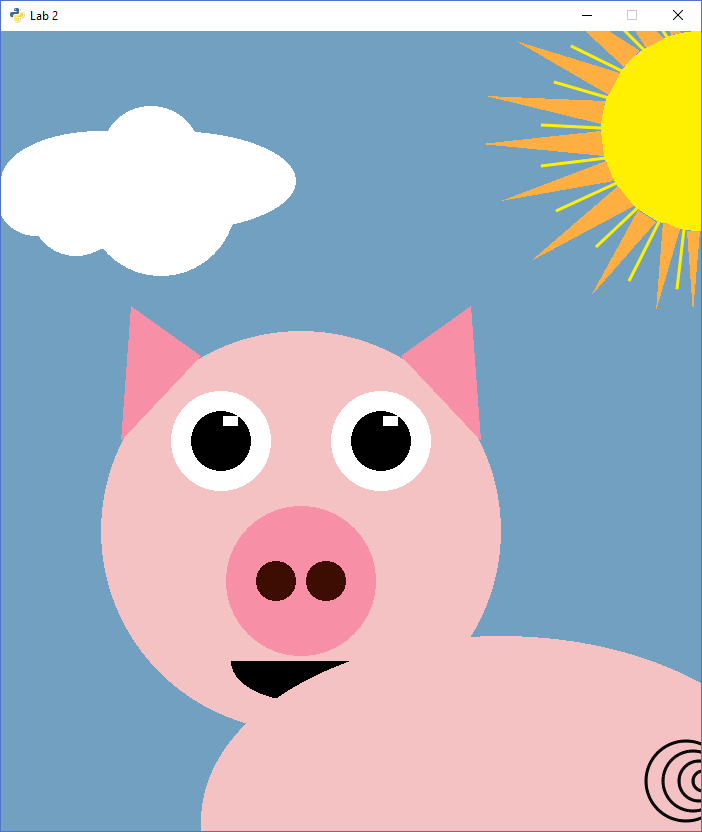
\includegraphics[height=.7\linewidth]{rita_gris}
  %\caption{1a}
  %\label{fig:gris}
\end{subfigure}%
\begin{subfigure}{.3\textwidth}
  \centering
  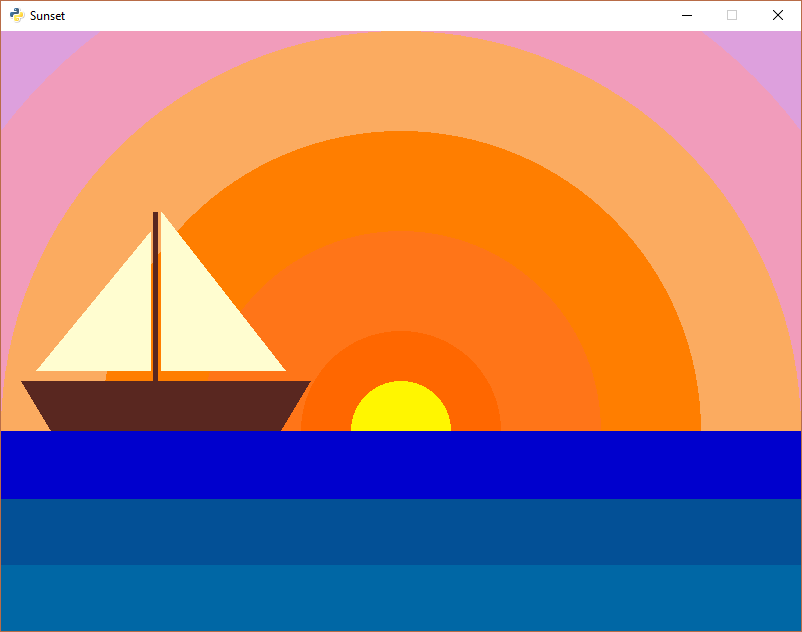
\includegraphics[height=.7\linewidth]{rita_solnedgang}
  %\caption{1b}
  %\label{fig:solnedgang}
\end{subfigure}%
\begin{subfigure}{.3\textwidth}
  \centering
  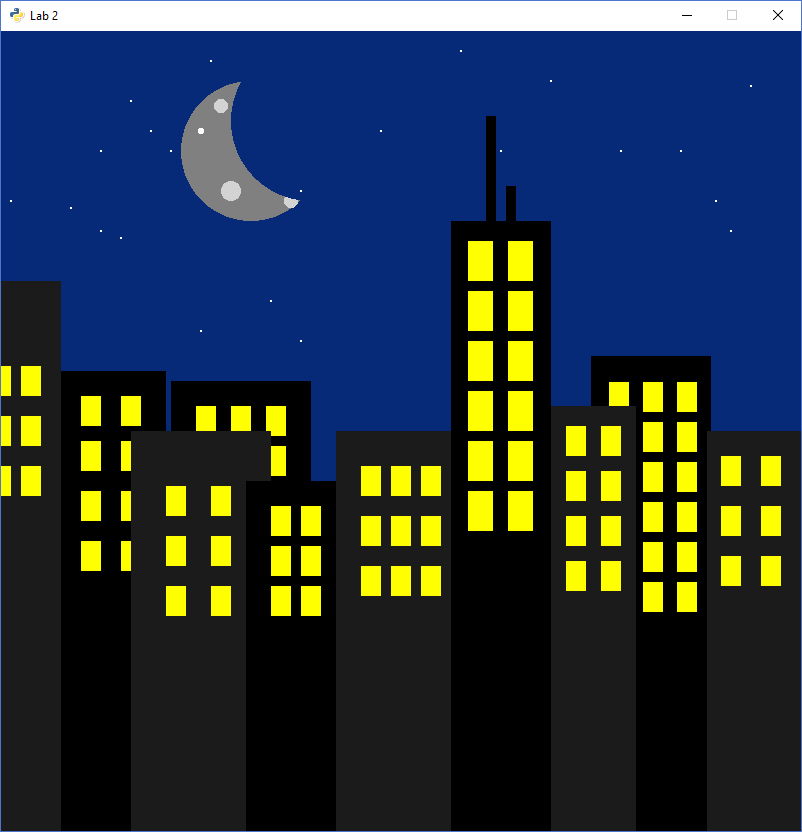
\includegraphics[height=.7\linewidth]{rita_stad}
  %\caption{1b}
  %\label{fig:stad}
\end{subfigure}
\caption{Exempel på vad man kan rita}
\label{fig:rita}
\end{figure}


Importera arcade i python-filen genom att skriva

\begin{lstlisting}
import arcade
\end{lstlisting}

och öppna ett fönster från arcade-biblioteket och skriv en titel. Välj Fönstrets dimensioner (bredd och höjd) och börja rita. Du kan bland annat använda dig av arcade-funktionerna nedanför.

\begin{lstlisting}
arcade.open_window(800, 600, "Titel") # öppnar ett fönster med bredd 800, höjd 600 och titel "Titel"
arcade.set_background_color(arcade.color.AFRICAN_VIOLET) # skapar en bakgrundsfärg
arcade.start_render() # gör sig redo för att börja rita

# rektangel som defineras utifrån x- och y-positionerna till rektangelns kanter. Först x-positionen till vänstra kanten (0), därefter x-positionen till högra kanten (800), sedan y-positionen till den övre kanten (200) och till sist y-positionen till den nedre kanten(0):
arcade.draw_lrtb_rectangle_filled(0, 800, 200, 0, arcade.color.BITTER_LIME)
# rektangel som defineras utifrån rektangelns centrum (x- och y-positionen (70,260)), följt av bredden (30) och höjden (40) till rektangeln:
arcade.draw_rectangle_filled(70, 260, 30, 40, arcade.color.BONE)
# triangel med hörnpositionerna (100, 470), (280, 470) och (190, 500):
arcade.draw_triangle_filled(100, 470, 280, 470, 190, 500, arcade.color.BROWN)
# polygon med hörnpositionerna (20,350),(100, 470),(280, 470) och (360, 340):
arcade.draw_polygon_filled([[20, 350],
                            [100, 470],
                            [280, 470],
                            [360, 340]],
                            arcade.color.BROWN)
# cirkel med centrum i (400,100) och radie 50:
arcade.draw_circle_filled(400, 100, 50, arcade.color.BLACK_OLIVE)


arcade.finish_render() # avslutar möjligheten att rita
arcade.run() # Låter fönstret vara öppet tills någon stänger det
\end{lstlisting}

Fönstrets origo (0,0) ligger i det nedre vänstra hörnet.\\
Du kan byta ut draw\_circle\_filled mot draw\_circle\_outline om du enbart vill ha kanterna till föremålet, istället för att den ska vara ifylld.
För att se vad färgerna heter kan du gå in på länken \url{http://arcade.academy/arcade.color.html} (namnen på färgerna i arcade) och \url{https://www.webpagefx.com/web-design/color-picker/color-chart/} (färgschema där man kan se hur färgerna ser ut). Du kan hitta fler geometriska former och rit-hjälpmedel på \url{http://arcade.academy/arcade.html#module-arcade.draw_commands}.


\begin{figure}[!ht]
\centering
\begin{subfigure}{.4\textwidth}
  \centering
  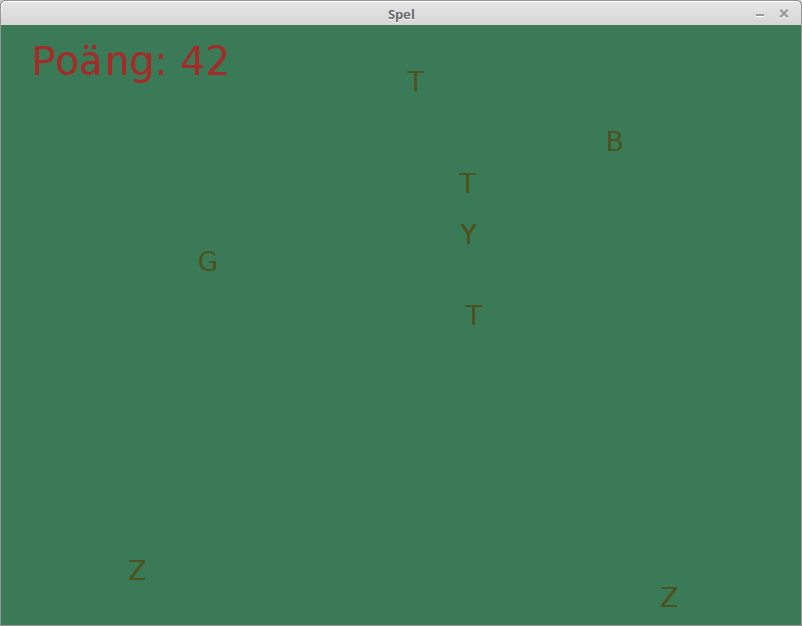
\includegraphics[width=\textwidth]{bokstavsspel}
  \caption{Bokstavsspel där man ska skriva snabbt.}
  %\label{fig:gris}
\end{subfigure}\quad%
\begin{subfigure}{.4\textwidth}
  \centering
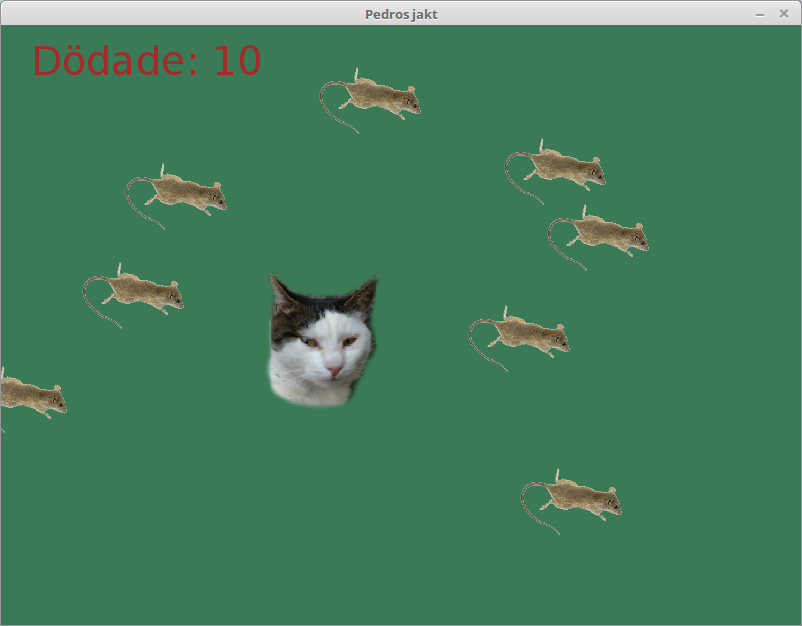
\includegraphics[width=\textwidth]{pedrospel}
\caption{Hjälp Pedro att döda alla möss.}
  %\label{fig:solnedgang}
\end{subfigure}
%\caption{Exempel på vad man kan rita}
%\label{fig:rita}
\end{figure}


\i Förbättra bokstavsspelet. Förslag:

\pu Öka hastigheten allt eftersom eller skapa fler och fler bokstäver, så det blir svårare för spelaren ju längre man spelar.

\pu Lägg till andra specialtecken på tangentbordet. Bokstäver med shift kräver en del trix, och å, ä, ö och några fler är krångliga, men testa siffror, punkt, komma, plus, bindestreck och liknande.

\pu Skriv ut Game Over i spelet istället för i terminalen. 

\pu Lägg till ljudeffekter.

\pu Lägg till möjligheten att starta om spelet (genom att klicka mellanslag?). 

\pu Få bokstäverna att gunga nedåt.


\i Förbättra Pedro-spelet. Förslag:

\pu Lägg till maximalt antal möss, och att det inte skapar möss när Pedro står still.

\pu Det ska inte kunna skapas möss på Pedro (åtminstone ska de inte ge poäng om de äts upp).

\pu Gör så att Pedro växer vid varje mumsbit.

\pu Få mössen att röra sig. Kanske är de rädda för Pedro och springer ifrån honom? 

\pu Lägg till något som Pedro ska undvika att äta, till exempel choklad.

\pu Lägg till Game Over

\pu Lägg till möjligheten att starta om spelet.

\pu Lägg till ljudeffekter.

\pu Begränsa Pedros rörelser med väggar och annat som den inte kan röra sig genom.

\i Skapa ett eget valfritt spel.

\url{https://kenney.nl} innehåller en hel del gratis paket med grafik och ljud för spel. Annars är google din vän. 






\end{document}